%!TEX root=../GaugeCNNTheory.tex


\subsection{مقدمه‌ای کوتاه بر کلاف‌های تاری}
\label{sec:fiber_bundles_general}


به طور شهودی، یک \emph{کلاف تاری} را می‌توان فضایی در نظر گرفت که با گرفتن یک فضای دیگر موسوم به \emph{فضای پایه}، در مورد ما خمینه $M$، و چسباندن فضای دیگری $F$ موسوم به \emph{تار}، به هر یک از نقاط آن ساخته می‌شود.
یک مثال بدیهی، حاصلضرب مستقیم \mbox{$M\times F$} خواهد بود.
با این حال، تارها به طور کلی می‌توانند به روشی پیچ‌خورده به هم متصل شوند، به طوری که کلاف حاصل از نظر توپولوژیکی با یک حاصلضرب متفاوت باشد.
\begin{wrapfigure}[13]{r}{0.54\textwidth}
	\vspace*{-1.4ex}
	\hfill
	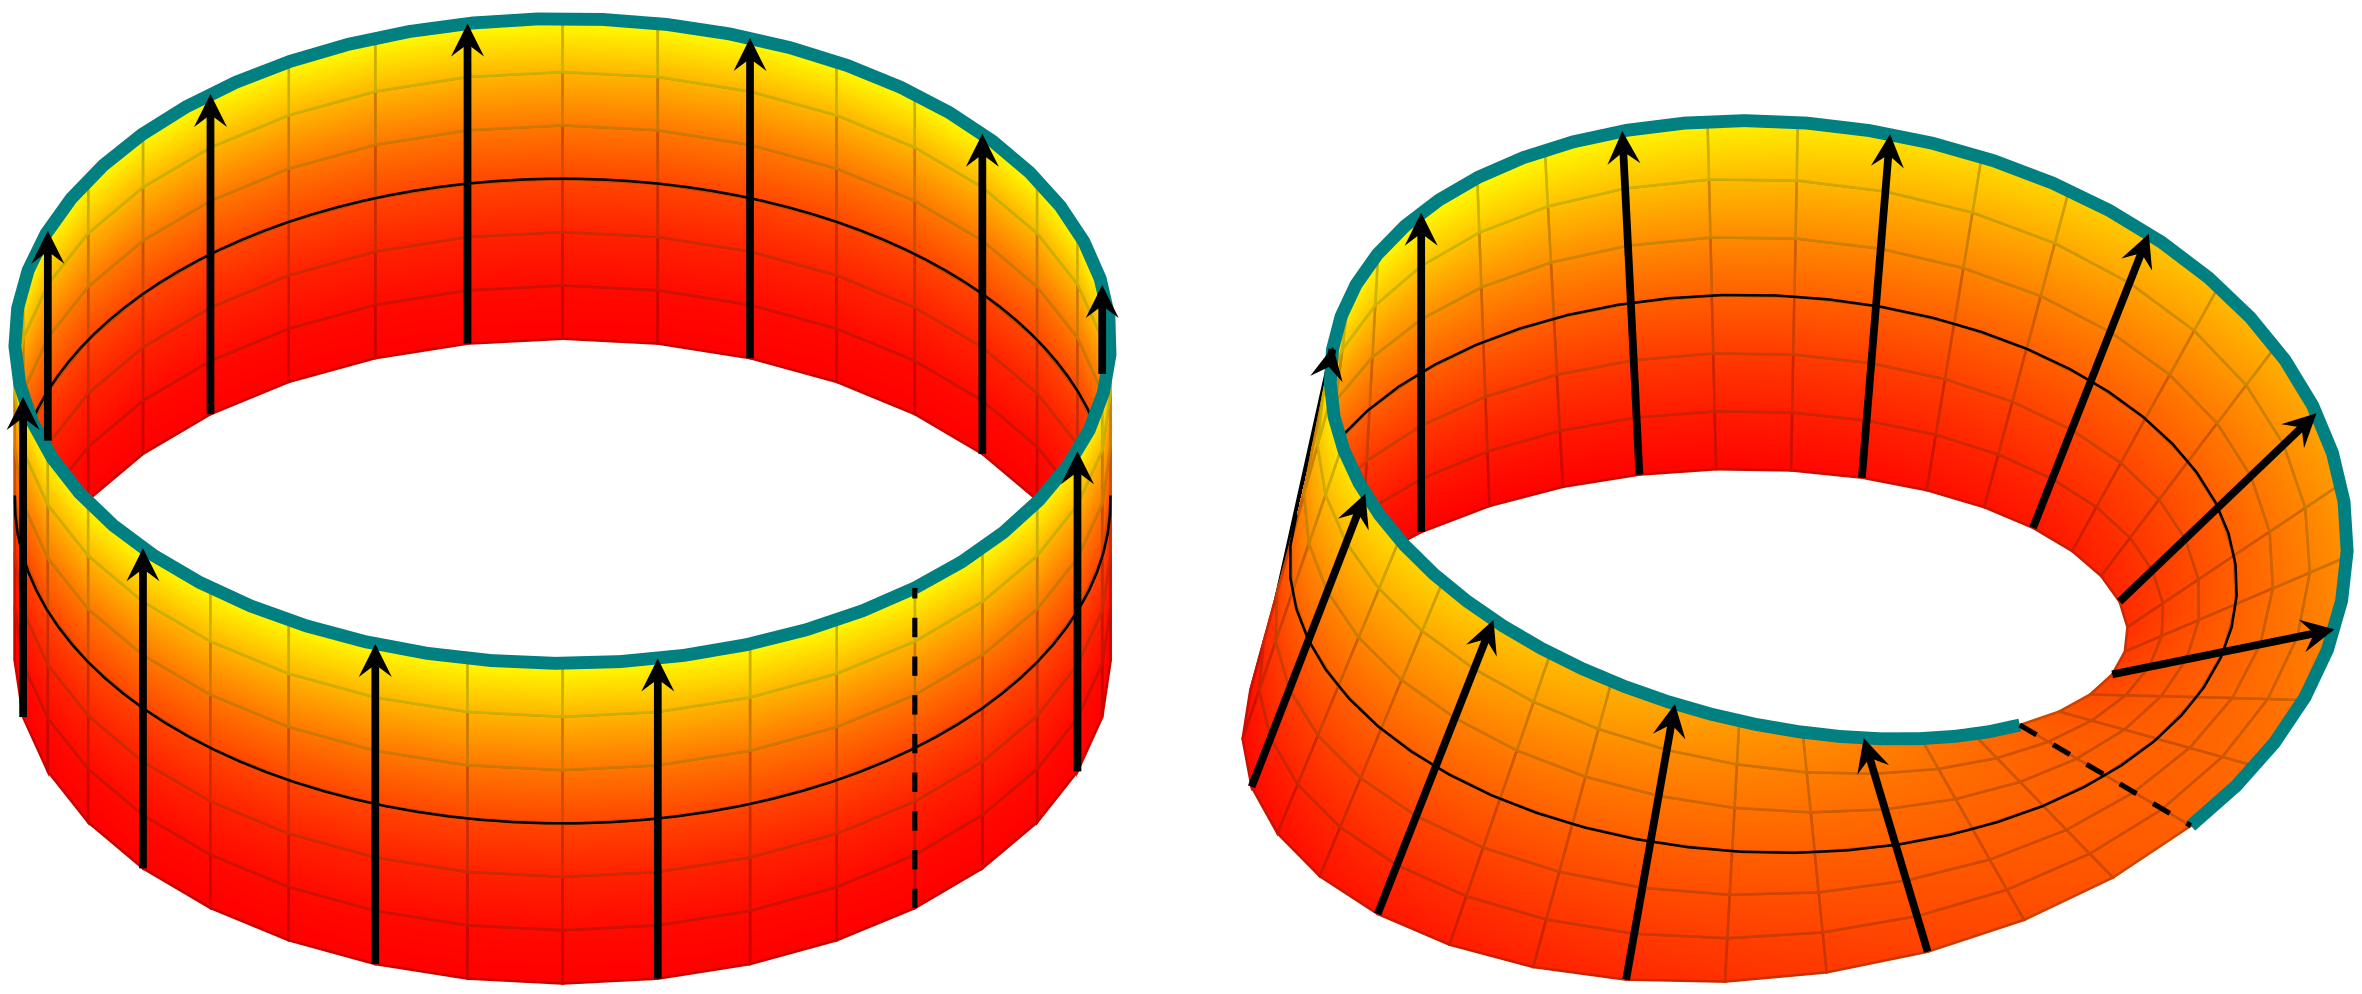
\includegraphics[width=.98\linewidth]{figures/moebius.png}%
	\vspace*{.2ex}
	\caption{\small
		یک استوانه و یک نوار موبیوس.
		هر دو کلاف، دایره $S^1$ را به عنوان فضای پایه و پاره‌خط‌های $[-1,1]$ را به عنوان تار مشترک دارند، با این حال، ساختار توپولوژیکی آنها به واسطه یک پیچش در تارها متفاوت است.
		{\\
			\color{gray}
			\scriptsize
			(شکل بر اساس کد جیک از
			\href{https://tex.stackexchange.com/questions/118563/moebius-strip-using-tikz}{\lr{\underline{tex.stackexchange.com}}}.)
		}
	}
	\label{fig:moebius}
\end{wrapfigure}%
به عنوان مثال، فرض کنید فضای پایه دایره $M=S^1$ و تار، پاره‌خط $F=[-1,1]$ باشد.
حاصلضرب مستقیم آنها $S^1\times[-1,1]$ یک استوانه را تشکیل می‌دهد؛ به شکل~\ref{fig:moebius} (چپ) مراجعه کنید.
در مقابل، اگر تارها به گونه‌ای چسبانده شوند که پس از یک دور کامل حول دایره، "وارونه" شوند، نوار موبیوس به دست می‌آید که یک کلاف تاری غیربدیهی است و از نظر توپولوژیکی با استوانه تفاوت دارد؛ به شکل~\ref{fig:moebius}~(راست) مراجعه کنید.%
\footnote{
	برای جلوگیری از سردرگمی، تأکید می‌کنیم که این مثال، نوار موبیوس را به عنوان یک کلاف تاری با فضای پایه (خمینه) $M=S^1$ در نظر می‌گیرد.
	در مقابل، تمام شکل‌های قبلی که شامل نوار موبیوس بودند، آن را به عنوان فضای پایه (خمینه) $M$ برای کانولوشن در نظر می‌گرفتند.
}%
\footnote{
	علاوه بر این، باید اشاره کنیم که پیکان‌های نشان داده شده در شکل فقط برای تأکید بر پیچش در نوار موبیوس هستند.
	آنها به معنای جهت چسباندن مانند \emph{نمودارهای چسباندن} \emph{نیستند}.
}
توجه داشته باشید که نوار موبیوس به صورت \emph{محلی} شبیه به حاصلضرب مستقیم $U\times F$ از یک جزء خطی $U\subsetneq S^1$ با تار~$F$ است.
همانطور که در ادامه بحث می‌شود، کلاف‌های تاری طبق تعریف همیشه می‌توانند به صورت محلی به حاصلضرب‌های مستقیم بدیهی‌سازی شوند.


ما به کلاف‌های تاری علاقه‌مندیم زیرا آنها امکان توصیف سراسری میدان‌ها روی خمینه‌ها را فراهم می‌کنند.
به عنوان مثال، یک میدان باد روی کره $M=S^2$ یک میدان برداری مماس است که به هر نقطه $p$ از~$M$ یک بردار مماس در $\TpM$ نسبت می‌دهد.
کلاف تاری متناظر، کلاف مماس $\TM$ است که تمام فضاهای مماس را به هم متصل می‌کند و بنابراین به عنوان یک کلاف تاری با فضای پایه $M=S^2$ و تار $\R^d\cong \TpM$ شناسایی می‌شود.
مشابه تارهای نوار موبیوس، فضاهای مماس یک خمینه خمیده به طور کلی به روشی کانونی به هم متصل نیستند، بلکه ذاتاً نسبت به یکدیگر پیچ خورده‌اند.
بنابراین، کلاف مماس به طور کلی از نظر توپولوژیکی با یک حاصلضرب متمایز است، یعنی $\TM \ncong M\times\R^d$.
به منظور تعریف میدان‌های برداری ویژگی $c$-بعدی، ما بعداً کلاف‌هایی با فضای پایه $M$ و فضاهای برداری ویژگی $\R^c$ به عنوان تار در نظر خواهیم گرفت.


\paragraph{کلاف‌های تاری به طور کلی:}
به طور رسمی، یک کلاف تاری ساختاری $(E,M,\pi,F)$ است که از فضاهای توپولوژیکی $E$ (فضای کلی)، $M$ (فضای پایه) و $F$ (تار نوعی) و یک نگاشت تصویر پیوسته و پوشا $\pi:E\to M$ تشکیل شده است.
یک کلاف تاری \emph{به صورت محلی بدیهی‌شدنی} است، به این معنی که برای هر نقطه $p\in M$ یک همسایگی محلی $U\subseteq M$ از~$p$ وجود دارد که کلاف، محدود به آن، شبیه به یک حاصلضرب مستقیم $U\times F$ است.
بدیهی بودن محلی توسط همسان‌ریختی‌ها%
\footnote{
	یک \emph{همسان‌ریختی} یک یکریختی توپولوژیکی است، یعنی یک نگاشت پیوسته و معکوس‌پذیر بین فضاهای توپولوژیکی با معکوس پیوسته.
}
$\Psi:\pi^{-1}(U)\to U\times F$ فرمول‌بندی می‌شود که نمودار جابجایی زیر را برآورده می‌کند:
\\[-2ex]
\begin{equation}\label{cd:trivialization_general_intro}
\begin{tikzcd}[row sep=3em, column sep=4em]
	\:E\: \supseteq
	&[-4.2em]
	\pi^{-1}(U) \arrow[d, swap, "\pi"] \arrow[r, "\Psi"]
	& U\times F \arrow[ld, "\proj_1"] \\
	M\, \supseteq
	& U
\end{tikzcd}
\quad ,
\end{equation}
یعنی،
\begin{align}\label{eq:local_triviality_proj}
	\pi\ =\  \proj_1 \circ \mkern2mu \Psi \,,
\end{align}
که در آن $\proj_1: U\times F\to U$ نگاشت تصویر طبیعی روی عامل اول را نشان می‌دهد.
کلافی که به صورت سراسری با حاصلضرب $M\times F$ همسان‌ریخت باشد، \emph{بدیهی} نامیده می‌شود.
کلاف‌ها اغلب به طور خلاصه به صورت $E\!\xrightarrow{\pi}\!M$ یا فقط $E$ نوشته می‌شوند و تار نوعی و فضای پایه به طور ضمنی فرض می‌شوند.
از آنجا که ما میدان‌های چارچوب هموار را در نظر می‌گیریم، فرض می‌کنیم $E$، $M$ و $F$ خمینه‌های هموار و $\pi$ و $\Psi$ نگاشت‌های هموار (دیفئومورفیسم) باشند.


بدیهی بودن محلی $E\!\xrightarrow{\pi}\!M$ ایجاب می‌کند که تصویر معکوس $E_p:=\pi^{-1}(p)$ از هر نقطه $p\in M$ که \emph{تار روی}~$p$ نامیده می‌شود، با تار نوعی $F$ دیفئومورف باشد.
همانند بخش~\ref{sec:gauge_cnns_intro_local}، ما دیفئومورفیسم‌هایی را که تارها روی نقاط مختلف را با تار نوعی یکی می‌دانند با $\psi_p:E_p\to F$ نشان می‌دهیم.
بدیهی‌سازی‌های محلی در این صورت بر حسب این دیفئومورفیسم‌ها به صورت زیر داده می‌شوند:
\begin{align}\label{eq:Psi_via_psi}
	\Psi:\pi^{-1}(U)\to U\times F,\ \ \ e\mapsto \big(\pi(e),\: \psi_{\pi(e)}(e)\big) \,.
\end{align}
اگر تار نوعی $F$ و تارهای $E_p$ روی $p$ ساختار اضافی داشته باشند، لازم است که دیفئومورفیسم‌های $\psi_p: E_p\to F$ این ساختار را حفظ کنند، یعنی یکریختی باشند.%
\footnote{
	به طور جایگزین، فرض کنید $F$ ساختاری دارد که توسط توابع گذار $\psi_p^B \circ (\psi_p^A)^{-1} = g^{BA}(p) \in \Aut(F)$ حفظ می‌شود (پاراگراف بعدی را ببینید).
	سپس بدیهی‌سازی‌های $\psi_p^X: E_p \to F$ به طور سازگار ساختار~$F$ را روی~$E_p$ \emph{القا} می‌کنند و به طور خودکار یکریختی هستند.
}
به عنوان مثال، اگر $F$ و $E_p$ ساختار فضای برداری داشته باشند، آنگاه $\psi_p$ باید خطی باشد.


به طور کلی، انتخاب خاص بدیهی‌سازی‌های محلی (یا دیفئومورفیسم‌ها) روی $U$ به طور کانونی توسط کلاف مشخص نمی‌شود.
بنابراین باید انتخاب‌های مختلف (پیمانه‌ها) و \emph{توابع گذار} (تبدیلات پیمانه) بین آنها را در نظر گرفت.
برای دقیق کردن این موضوع، دو همسایگی بدیهی‌ساز همپوشان $U^A$ و $U^B$ را با بدیهی‌سازی‌های محلی $\Psi^A$ و $\Psi^B$ در نظر بگیرید.
از معادله~\eqref{eq:Psi_via_psi} نتیجه می‌شود که گذار بین هر دو بدیهی‌سازی محلی روی $U^{AB}:=U^A\cap U^B\neq\varnothing$ به صورت زیر داده می‌شود:
\begin{align}\label{eq:transition_function_general_bdl}
	\Psi^B\!\circ\!\big(\Psi^A\big)^{-1}\!:\ U^{AB}\times F \to U^{AB}\times F,
	\quad (p,\mathscr{f}) \mapsto \left(p,\, \pig[\psi_p^B \!\circ\! \big(\psi_p^A\big)^{-1}\, \pig]\mkern-1.5mu(\mathscr{f}) \right)
	=: \left(p,\: g_p^{BA} \,\btr\mkern1.5mu \mathscr{f}\right)
\end{align}
که در آن ما به طور ضمنی \emph{توابع گذار} هموار را تعریف کردیم:%
\footnote{
	گروه خودریختی‌های $\operatorname{Aut}(F)$ یک فضا~$F$ از تمام نگاشت‌های معکوس‌پذیر و حافظ ساختار (یکریختی‌ها) از~$F$ به خودش تشکیل شده است.
	به عنوان مثال، اگر $F=\R^n$ یک فضای برداری باشد، گروه خودریختی، گروه خطی عام $\GL{n}$ است که از تمام ماتریس‌های معکوس‌پذیر $n\!\times\!n$ تشکیل شده است.
}
\begin{align}\label{eq:transition_functions_psi}
	g^{BA}: U^{AB} \to \Aut(F),\ \ \ p \mapsto g_p^{BA} := \psi_p^B \circ \big(\psi_p^A\big)^{-1}
\end{align}
و عمل چپ آنها
\begin{align}\label{eq:gauge_trafo_leftaction}
	\blacktriangleright\,:\, \Aut(F) \times F\to F, \quad
	\left(g_p^{BA}, \mathscr{f}\right) \;\mapsto\; g_p^{BA}\,\btr\mkern1.5mu \mathscr{f} \;:=\; \left[\psi_p^B\circ\big(\psi_p^A\big)^{-1}\right]\!(\mathscr{f}).
\end{align}
روی تار نوعی $F$؛ مقایسه کنید با معادلات~\eqref{eq:gauge_trafo_local_def_21} و~\eqref{eq:transition_fct_local_def_21}.
برای اینکه ببینیم عامل اول در معادله~\eqref{eq:transition_function_general_bdl} در واقع با همانی داده می‌شود، توجه داشته باشید که برای هر $p\in U^{AB}$ و هر $\mathscr{f}\in F$، اعمال مکرر معادله~\eqref{eq:local_triviality_proj} ایجاب می‌کند:
$
	\pig[ \proj_1 \circ \Psi^B \circ \big(\Psi^A\big)^{-1} \mkern1mu\pig] (p,\mathscr{f})
	\ =\ \pig[ \pi \circ \big(\Psi^A\big)^{-1}  \mkern1mu\pig] (p,\mathscr{f})
	\ =\ \proj_1 (p,\mathscr{f})
	\ =\ p \,.
$
گذار بین بدیهی‌سازی‌های مختلف توسط بسط (جابجایی) زیر از نمودار جابجایی در معادله~\eqref{cd:trivialization_general_intro} به تصویر کشیده شده است:
\begin{equation}\label{cd:trivialization_general_trafo}
\begin{tikzcd}[row sep=3.5em, column sep=5.em]
	U^{AB}\!\times\!F
		\arrow[rd, "\proj_1"']
		\arrow[rr, rounded corners, to path={ 
				-- ([yshift=4ex]\tikztostart.north) 
				--node[above, pos=.5]{\small$\id \times g^{BA}\btr$} ([yshift=4ex]\tikztotarget.north) 
				-- (\tikztotarget.north)
				}]
	& \pi^{-1}(U^{AB})
		\arrow[d, swap, "\pi"]
		\arrow[l, "\Psi^A"']
		\arrow[r, "\Psi^B"]
	& U^{AB}\!\times\!F
		\arrow[ld, "\proj_1"]
	\\
	& U^{AB}
\end{tikzcd}
\end{equation}
محدود به یک نقطه $p\in U^{AB}$، و برای حالت خاص کلاف مماس (که در ادامه تعریف می‌شود)، این نمودار با نمودار در معادله~\eqref{eq:commutative_diagram_TpM} و نسخه گرافیکی آن در شکل~\ref{fig:gauge_trafos} مطابقت دارد.


طبق تعریف، توابع گذار در معادله~\eqref{eq:transition_functions_psi} سه شرط زیر را برآورده می‌کنند:%
\footnote{%
	شرایط $i)$ و $ii)$ از شرط هم‌زنجیر $iii)$ نتیجه می‌شوند اما اغلب به طور صریح بیان می‌شوند.
}
\begin{alignat}{3}
	   i) \qquad&& g_p^{AA}    \;&=\ e                      \quad&&\forall p\in U^A \label{eq:transition_condition_1}\\
	  ii) \qquad&& g_p^{BA}    \;&=\big(g_p^{AB}\big)^{-1} \quad&&\forall p\in U^A\cap U^B \label{eq:transition_condition_2}\\
	 iii) \qquad&& g_p^{CB} g_p^{BA}\;&=\ g_p^{CA}            \quad&&\forall p\in U^A\cap U^B\cap U^C \qquad \text{(شرط هم‌زنجیر)} \label{eq:transition_condition_3}
\end{alignat}
طبق \emph{قضیه ساخت کلاف تاری}، هر کلاف تاری را می‌توان به طور کامل و سراسری بر حسب یک \emph{اطلس}
$\mathscr{A}\ =\ \big\{\big( U^X, \Psi^X \big) \,\big|\, X\in\mathfrak{X} \big\}$
از بدیهی‌سازی‌های محلی $\big(U^X,\Psi^X\big)$ مشخص کرد که $M$ را می‌پوشانند و توابع گذار آنها معادلات~\eqref{eq:transition_condition_1}، \eqref{eq:transition_condition_2} و~\eqref{eq:transition_condition_3} را برآورده می‌کنند (در اینجا $\mathfrak{X}$ یک مجموعه اندیس را نشان می‌دهد).
می‌توان بدیهی‌سازی‌های منفرد را به گونه‌ای تصور کرد که توسط نگاشت‌های گذار "به هم چسبیده‌اند"، که در شکل~\ref{fig:trivializations_moebius} به تصویر کشیده شده است.
توجه داشته باشید که این مشابه توصیف سراسری یک خمینه بر حسب یک اطلس از چارت‌های محلی است.


\paragraph{کلاف‌های برداری:}
چندین مفهوم خاص‌تر از کلاف‌های تاری وجود دارد که ساختار ریاضی اضافی دارند.
یک مثال مهم \emph{کلاف‌های برداری} هستند که همانطور که از نامشان پیداست، کلاف‌هایی هستند که از فضاهای برداری متصل به یک خمینه تشکیل شده‌اند.
به طور رسمی، یک کلاف برداری (حقیقی) از رتبه~$k$ یک کلاف $(E,M,\pi,\R^k)$ با تار نوعی~$\R^k$ و تارهای $E_p \cong \R^k$ روی $p$ است، به طوری که بدیهی‌سازی‌های محلی به ازای هر تار، یکریختی‌های فضای برداری (نگاشت‌های خطی) هستند.
توابع گذار $\psi^B_p \circ \big(\psi^A_p\big)^{-1} \in \Aut(\R^k) = \GL{k}$ در این صورت مقادیری در گروه خطی عام می‌گیرند.

به طور جایگزین، با داشتن تار $\R^k$ و یک اطلس از بدیهی‌سازی‌های محلی که توابع گذار آن مقادیری در $\Aut(\R^k) = \GL{k}$ می‌گیرند، یک ساختار فضای برداری برای $E_p$ با قرار دادن
\begin{align}
	\alpha v + \beta w \ :=\ \big(\psi_p^A \big)^{-1} \big( \alpha \psi_p^A(v) + \beta \psi_p^A(w) \big) \qquad \forall\ v,w\in E_p,\ \ \alpha,\beta\in\R
\end{align}
برای یک پیمانه دلخواه $\psi_p^A: E_p \to \R^k$ از اطلس $\GL{k}$ القا می‌شود.
اینکه ساختار فضای برداری به طور سازگار تعریف شده است واضح است زیرا
\begin{align}
		&\big( \psi_p^B \big)^{-1} \pig( \alpha \psi_p^B(v) + \beta \psi_p^B(w) \pig) \notag \\
	=\ &\big( \psi_p^A \big)^{-1} \pig( \big(g^{BA}_p)^{-1} \big( \alpha g^{BA}_p \psi_p^A(v) + \beta g^{BA}_p \psi_p^A(w) \big) \pig) \notag \\
	=\ &\big( \psi_p^A \big)^{-1} \pig( \alpha \psi_p^A(v) + \beta \psi_p^A(w) \pig)
\end{align}
همان نتیجه را به دست می‌دهد.
توجه داشته باشید که مرحله آخر نیازمند خطی بودن $g_p^{BA} \in \GL{d}$ بود.
پیمانه‌های $\psi_p^A$ یا $\psi_p^B$ در این صورت به طور خودکار یکریختی‌های فضای برداری هستند.

مهم‌ترین مثال‌ها برای ما کلاف مماس و کلاف‌های برداری ویژگی هستند که در بخش‌های بعدی معرفی می‌شوند.

\paragraph{\lr{\textit{G}}-کلاف‌ها}
بسته به توپولوژی کلاف، ممکن است بتوان یک اطلس از بدیهی‌سازی‌های محلی
$\mathscr{A}^G\ =\ \big\{\big( U^X, \Psi^X \big) \,\big|\, X\in\mathfrak{X} \big\}$
تعریف کرد که \emph{توابع گذار آن به یک زیرگروه ${G \leq \Aut(F)}$ محدود شده‌اند}، یعنی برآورده می‌کنند:
\begin{align}
	g_p^{BA} \in G\quad\ \ \textup{برای تمام}\ \ A,B\in\mathfrak{X}\ \ \textup{و تمام}\ \ p\in U^A\cap U^B \,.
\end{align}
هر چنین اطلسی، اطلس $G$ نامیده می‌شود و $G$ به عنوان \emph{گروه ساختار} کلاف شناخته می‌شود.
دو اطلس $G$ مختلف معادل (یا سازگار) هستند، اگر اجتماع آنها دوباره یک اطلس $G$ باشد.
کلافی که به یک کلاس هم‌ارزی از اطلس‌های $G$ مجهز شده باشد، به عنوان یک \lr{G}-کلاف شناخته می‌شود.%
\footnote{
	کلاس هم‌ارزی تضمین می‌کند که هیچ یک از اطلس‌های $G$ معادل، برتری ندارند.
	به طور معادل، می‌توان اطلس $G$ \emph{ماکسیمال} را در نظر گرفت که به عنوان اطلس $G$ منحصربه‌فردی تعریف می‌شود که هر اطلس $G$ سازگار دیگری در آن موجود است.
	توجه داشته باشید که یک کلاس هم‌ارزی از اطلس‌های $G$ به طور منحصربه‌فرد توسط یک اطلس $G$ داده شده، ایجاب می‌شود.
}

\begin{figure*}
	\centering
	\begin{subfigure}[b]{0.46\textwidth}
		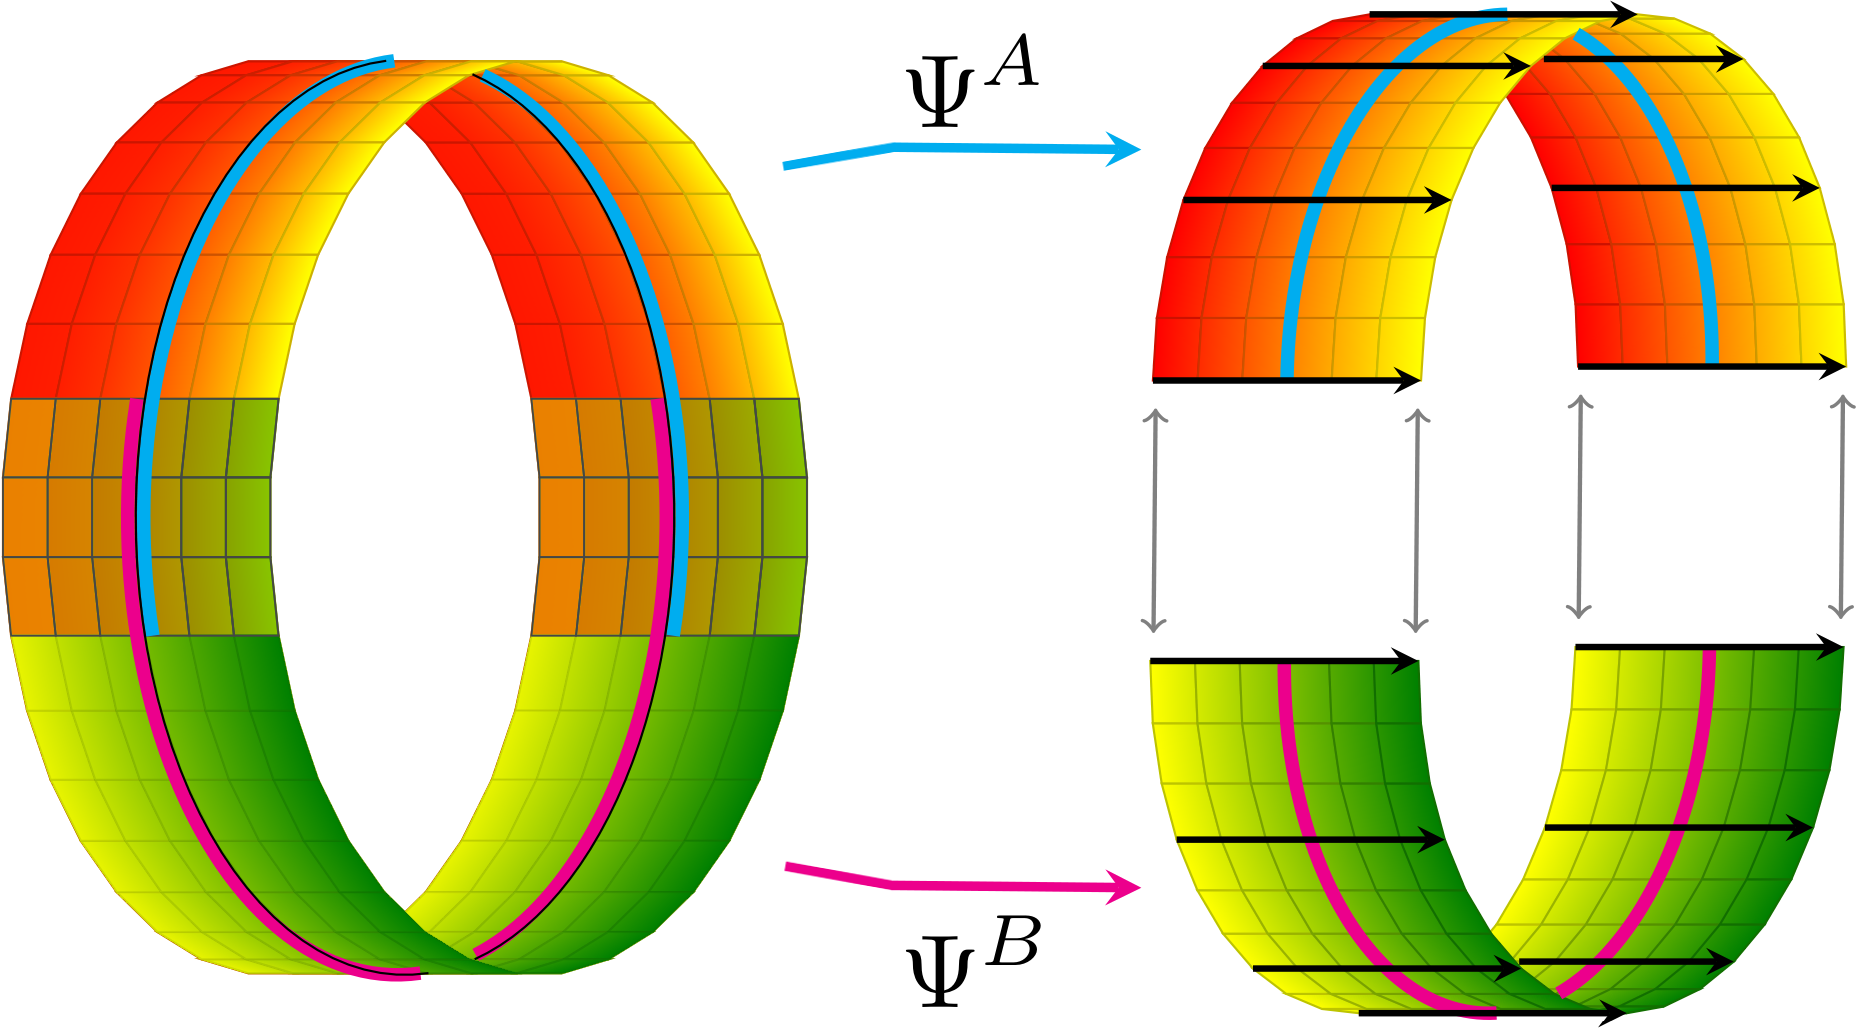
\includegraphics[width=\textwidth]{figures/trivialization_cylinder.png}
	\end{subfigure}
	\hfill
	\begin{subfigure}[b]{0.46\textwidth}
		\centering
		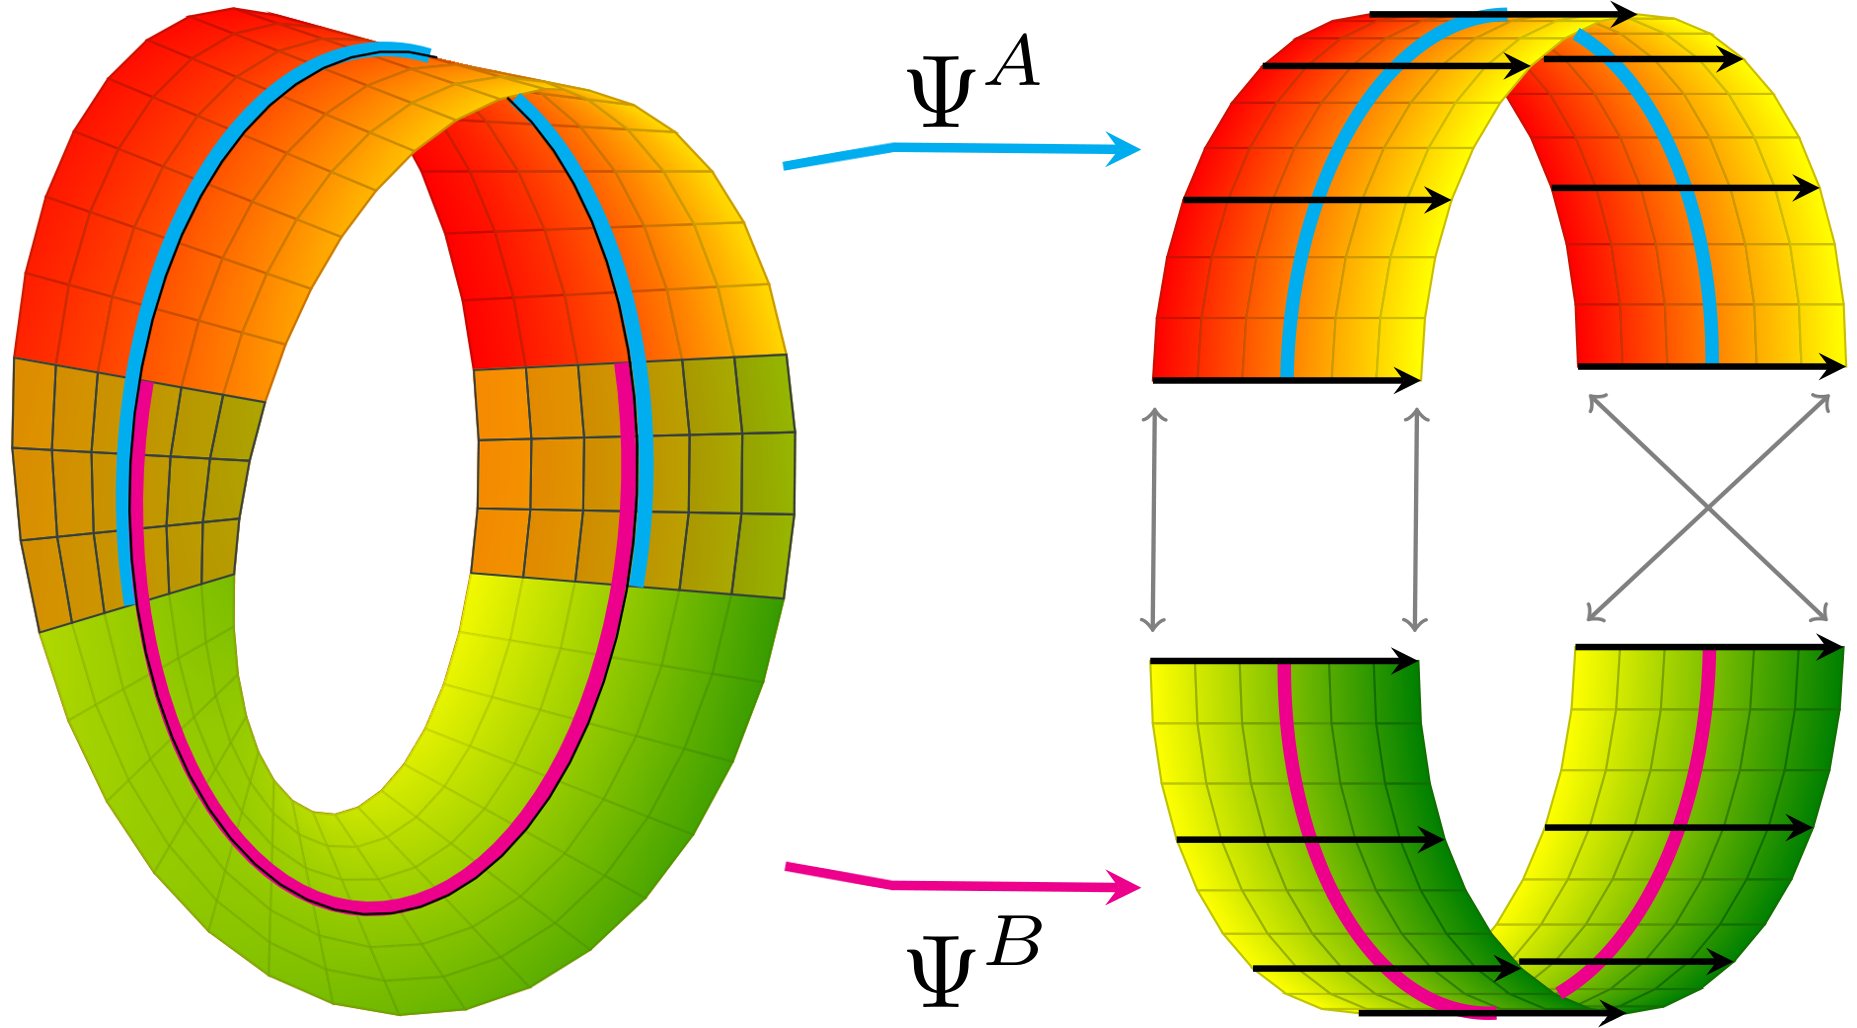
\includegraphics[width=\textwidth]{figures/trivialization_moebius_2.png}
	\end{subfigure}
	\vspace{2.ex}
	\caption{\small
		توصیف استوانه و نوار موبیوس بر حسب اطلس‌های $G$ که هر کدام از دو بدیهی‌سازی محلی تشکیل شده‌اند.
		\textit{چپ:}~از آنجا که استوانه یک کلاف بدیهی است، تمام توابع گذار را می‌توان به عنوان نگاشت‌های همانی انتخاب کرد به طوری که گروه ساختار به گروه بدیهی $G=\{e\}$ کاهش یابد.
		برخلاف وضعیت به تصویر کشیده شده، امکان انتخاب یک بدیهی‌سازی سراسری و واحد وجود دارد.
		\textit{راست:}~توپولوژی نوار موبیوس توابع گذار را در یکی از همپوشانی‌ها مجبور می‌کند که تارها را به روشی وارونه به هم بچسبانند.
		بنابراین گروه ساختار را نمی‌توان بیشتر از گروه $G=\Flip$ که بازتاب تارها را مدل می‌کند، کاهش داد.
		بنابراین بدیهی‌سازی‌های سراسری برای نوار موبیوس وجود ندارد.
		توجه داشته باشید که پیکان‌های روی نوار موبیوس را نباید با پیکان‌های نمودارهای چسباندن اشتباه گرفت، یعنی پیچش، بردارها را در یکی از برش‌ها در جهت مخالف می‌چسباند.
	}
	\label{fig:trivializations_moebius}
\end{figure*}

توپولوژی یک کلاف تعیین می‌کند که گروه ساختار آن تا چه حد قابل کاهش است.
به عنوان مثال، استوانه در شکل~\ref{fig:trivializations_moebius} (یا هر کلاف بدیهی دیگر) را می‌توان با یک اطلس $\{e\}$ توصیف کرد که فقط از بدیهی‌سازی‌های محلی با توابع گذار همانی تشکیل شده است.
این متناظر با کاهش به یک گروه ساختار بدیهی $G=\{e\}$ است.
در مقابل، توپولوژی پیچ‌خورده نوار موبیوس ایجاب می‌کند که هر اطلس $G$ شامل توابع گذاری باشد که تارها را با جهت‌گیری وارونه به هم بچسبانند؛ به شکل~\ref{fig:trivializations_moebius} (راست) مراجعه کنید.
بنابراین گروه ساختار نوار موبیوس را نمی‌توان بیشتر از گروه $G=\Flip$ که بازتاب تارها را مدل می‌کند، محدود کرد.
روی خمینه‌های ریمانی، گروه ساختار کلاف مماس $\TM$ و در نتیجه کلاف‌های برداری ویژگی وابسته، به طور کلی نمی‌توانند بیشتر از یک گروه ساختار متعامد $\O{d}$ کاهش یابند، که این کار روی CNNهای مستقل از مختصات را در وهله اول انگیزه‌مند کرد.

\paragraph{کلاف‌های \lr{\textit{G}} وابسته:}
دو \lr{G}-کلاف را \emph{وابسته} به یکدیگر می‌نامند اگر دارای فضای پایه، گروه ساختار و مهمتر از همه، \emph{توابع گذار یکسان} باشند.
کلاف‌های وابسته $(E,M,\pi,F)$ و $(\widetilde{E},M,\widetilde{\pi},\widetilde{F})$ با گروه ساختار $G$ ممکن است در تارهای نوعی خود~$F$ و $\widetilde{F}$ و بنابراین در عمل چپ $\blacktriangleright: G \times F\to F$ و $\widetilde{\blacktriangleright}: G \times \widetilde{F}\to \widetilde{F}$ گروه~$G$ بر روی تار مربوطه متفاوت باشند.
با داشتن دو اطلس $G$
$\big\{\big( U^X,              \Psi^X  \big) \,\big|\, X\in\mathfrak{X} \big\}$ و
$\big\{\big( U^X, \widetilde{\Psi}^X \big) \,\big|\, X\in\mathfrak{X} \big\}$
از کلاف‌ها روی همان پوشش باز از $M$ ، شرط هم‌ارزی توابع گذار (تا حد عمل‌های چپ مختلف) به این معنی است:
\begin{align}
	\Psi^B \circ \big(\Psi^A \big)^{-1}\ =\ \big(\id \times g^{BA}\blacktriangleright \big)
	\qquad \Longleftrightarrow \qquad
	\widetilde{\Psi}^B \circ \big(\widetilde{\Psi}^A \big)^{-1}\ =\ \big(\id \times g^{BA}\, \widetilde{\blacktriangleright} \big)
\end{align}
به طور شهودی، تارهای نوعی~$F$ و~$\widetilde{F}$ از~$E$ و~$\widetilde{E}$ به روشی یکسان روی~$M$ "به هم چسبیده‌اند".

یک مثال مهم از کلاف‌هایی که به صورت $\GL{d}$-وابسته به یکدیگر هستند، کلاف مماس $\TM$، کلاف هم‌مماس $\TsM$، هر کلاف تانسوری دیگر $\TrsM$ و کلاف چارچوب مماس~$\FM$ هستند (اولی و آخری در بخش~\ref{sec:GL_associated_bundles} معرفی شده‌اند).
وابستگی این کلاف‌ها در این واقعیت منعکس می‌شود که مؤلفه‌های آنها نسبت به پایه‌های انتخاب شده مطابق با همان تبدیل پیمانه تبدیل می‌شوند (مثلاً ژاکوبین $g^{BA}_{\mu\nu} = \frac{\partial x^B_\mu}{\partial x^A_\nu}$، به پیوست~\ref{apx:coordinate_bases} مراجعه کنید).
عمل‌های مختلف یک تبدیل پیمانه بر روی تارهای مربوطه در این مثال به عنوان تبدیل پادوردا ($\TM$)، تبدیل هموردا ($\TsM$)، تبدیل $r$-بار پادوردا و $s$-بار هموردا ($\TrsM$) و دوباره، تبدیل هموردا ($\FM$)، به ترتیب، مشخص می‌شوند.
ما بعداً ساختار $G$ $\GM$، کلاف مماس $\TM$ و کلاف‌های برداری ویژگی $\A$ را به عنوان کلاف‌های $G$ وابسته معرفی خواهیم کرد.
وابستگی در این مورد از این واقعیت ناشی می‌شود که تغییرات چارچوب‌های مرجع در $\GM$ منجر به تبدیل همزمان ضرایب بردار مماس و ضرایب بردار ویژگی می‌شود.

می‌خواهیم اشاره کنیم که هر کلاف وابسته‌ای علاوه بر این به یک کلاف اصلی $G$ منحصربه‌فرد (که در پاراگراف بعدی تعریف می‌شود) وابسته است.
در مقابل، هر کلاف وابسته را می‌توان از کلاف اصلی وابسته مربوطه ساخت -- ما از این ساختار به طور گسترده برای تعریف کلاف‌های برداری ویژگی در بخش~\ref{sec:G_associated_bundles} استفاده خواهیم کرد.

\paragraph{کلاف‌های اصلی \lr{\textit{G}}:}
یک کلاف تاری $(P,M,\pi,G)$ را یک \emph{کلاف اصلی (هموار) $G$} $(P,M,\pi,G,\lhd)$ می‌نامند اگر ۱) تار نوعی آن با گروه ساختار آن $G$ منطبق باشد و ۲) به یک \emph{عمل راست (هموار) $G$}
\begin{align}
	\lhd: P \times G \to G,\ \ (\mathscr{p},g) \mapsto \mathscr{p}\lhd g
\end{align}
مجهز باشد که تارها را حفظ می‌کند، یعنی،
\begin{align}
	\pi(\mathscr{p}\lhd g)\ =\ \pi(\mathscr{p})\quad \forall\ \mathscr{p}\in P,\ g\in G
\end{align}
و به صورت \emph{تعدی‌پذیر} و \emph{آزاد} روی آنها عمل می‌کند.%
\footnote{%
	یک عمل گروهی (راست) $\phi:X\times G\to X,\ (x,g)\mapsto x.g$ را \emph{تعدی‌پذیر} می‌نامند اگر هر نقطه از $X$ را بتوان به هر نقطه دیگر نگاشت، یعنی اگر برای هر $x,y\in X$ یک $g\in G$ وجود داشته باشد به طوری که $y=x.g$.
	آن را (نقطه ثابت) \emph{آزاد} می‌نامند اگر برای هر $x\in X$ معادله $x=x.g$ ایجاب کند که $g=e$ باشد، یعنی اگر تنها عمل عنصر همانی $p$ را ناوردا باقی بگذارد.
	توجه داشته باشید که همین گزاره‌ها را می‌توان برای عمل‌های چپ نیز بیان کرد.
}
دو شرط آخر (تعدی‌پذیری و آزادی) با هم ایجاب می‌کنند که تارهای یک کلاف اصلی $G$ ، $G$-تورسور (یا فضاهای همگن اصلی $G$) باشند، که به طور شهودی به این معناست که آنها "شبیه به~$G$" هستند اما بدون هیچ مبدأ یا عنصر همانی مشخصی ارائه می‌شوند.%
\footnote{
	به طور رسمی، یک $G$-تورسور (راست) $P$ شرط $P\times G \cong P\times P$ را برآورده می‌کند که در آن یکریختی توسط $(p,g) \mapsto (p,p.g)$ داده می‌شود.
	این شرط ایجاب می‌کند که یک عنصر گروهی \emph{منحصربه‌فرد} وجود داشته باشد که \emph{هر} دو نقطه در تورسور را به هم متصل کند.
}
بدیهی‌سازی‌های محلی $\Psi: \pi^{-1}(U) \to U \times G$ باید عمل راست $G$ را حفظ کنند، یعنی هموردای راست $G$ باشند:
\begin{align}\label{eq:right_G_equiv_principal_bdl_general}
	\Psi(\mathscr{p} \lhd g)\ =\ \Psi(\mathscr{p}) (\id \times \cdot\mkern1mu g)
	\quad \textup{یا، به طور معادل،}\quad
	\psi_{\pi(\mathscr{p})} (\mathscr{p}\lhd g)\ =\ \psi_{\pi(\mathscr{p})} (\mathscr{p}) \cdot\mkern0mu g
	\qquad \forall\ \mathscr{p}\in P,\ g\in G \,,
\end{align}
که در آن $\cdot g$ ضرب راست کانونی با عناصر گروه روی تار نوعی~$G$ را نشان می‌دهد.
این، نمودار در معادله~\eqref{cd:trivialization_general_intro} را به نمودار زیر بسط می‌دهد:
\begin{equation}\label{cd:trivialization_principal_intro}
\begin{tikzcd}[row sep=3.5em, column sep=4.5em]
	% Row 1
	  \pi^{-1}(U)
			\arrow[r, "\Psi"]
	& U\times G
	\\
	% Row 2
	  \pi^{-1}(U)
			\arrow[d, "\pi\,"']
			\arrow[r, "\Psi"]
			\arrow[u, "\lhd g\ "]
	& U\times G
			\arrow[ld, "\proj_1"]
			\arrow[u, "\ (\id \times \cdot g)"']
	\\
	% Row 3
	U
\end{tikzcd}
\quad,
\end{equation}
که لازم است برای هر $g\in G$ جابجا باشد.

کلاف‌های اصلی $G$ برای مطالعه کلاف‌های عمومی $G$ از اهمیت زیادی برخوردارند.
به طور خاص، هر کلاف $G$ $(E,M,\pi_E,F)$ به یک کلاف اصلی $G$ (منحصربه‌فرد) $(P,M,\pi_P,G,\lhd)$ روی~$M$ وابسته است و هر کلاف $G$ وابسته را می‌توان از $P$ ساخت.
در بخش‌های بعدی، ما کلاف چارچوب~$\FM$ و $G$-ساختارها~$\GM$ را به عنوان نمونه‌های خاصی از کلاف‌های اصلی ارائه خواهیم داد، که ادعاهای مطرح شده در اینجا را کمتر انتزاعی کرده و برخی از پیامدهای آنها را آشکار می‌سازد.

\paragraph{برش‌ها و میدان‌ها:}
میدان‌های هموار با مقدار $F$ روی $M$ به عنوان \emph{برش‌های} هموار $\sigma$ از یک کلاف $E\!\xrightarrow{\pi}\!M$ با تار $F$ فرمول‌بندی می‌شوند.
یک برش هموار در این صورت به عنوان یک نگاشت هموار $\sigma:M\to E$ تعریف می‌شود که به هر نقطه $p$ از فضای پایه یک عنصر در تار $E_p$ روی $p$ نسبت می‌دهد، یعنی شرط $\pi\circ\sigma=\id_M$ را برآورده می‌کند، که نمودار جابجایی زیر آن را به تصویر می‌کشد:
\begin{equation}\label{cd:section_proj_idM}
\begin{tikzcd}[row sep=3em, column sep=4.5em]
	  M \arrow[r, "\sigma"]
		\arrow[rr, rounded corners, to path={ 
				-- ([yshift=-3.ex]\tikztostart.south) 
				--node[below, pos=.5]{\small$\id_M$} ([yshift=-3.ex]\tikztotarget.south) 
				-- (\tikztotarget.south)
				}]
	& E \arrow[r, "\pi"]
	& M
\end{tikzcd}
\end{equation}
یک مثال مهم میدان‌های برداری مماس هستند که به عنوان برش‌های $v: M\to \TM$ مدل می‌شوند که به هر نقطه $p$ در $M$ یک بردار مماس $v(p)\in \TpM$ نسبت می‌دهند.
توجه داشته باشید که نگاشت تصویر، به طبیعت خود، معکوس‌ناپذیر است، به طوری که $\sigma\circ\pi\neq\id_E$.
بنابراین نمودار زیر به طور کلی جابجا \emph{نمی‌شود}:
\begin{equation}\label{cd:section_proj_noncommutative}
\begin{tikzcd}[row sep=3em, column sep=4.5em,
			   execute at end picture={
					\node [] at (-.04, -.46) {$\noncommutative$};
					}]
	  E \arrow[r, "\pi"]
		\arrow[rr, rounded corners, to path={ 
				-- ([yshift=-3.5ex]\tikztostart.south) 
				--node[below, pos=.5]{\small$\id_E$} ([yshift=-3.5ex]\tikztotarget.south) 
				-- (\tikztotarget.south)
				}]
	& M \arrow[r, "\sigma"]
	& E
\end{tikzcd}
\end{equation}
در مواردی که در ادامه یک نمودار جابجا نباشد، که بیشتر در مورد برش‌ها صدق می‌کند، ما این موضوع را با افزودن نماد $\raisebox{-2pt}{\noncommutative}$ به صورت بصری تأکید می‌کنیم.
برش‌های هموار لزوماً به صورت سراسری وجود ندارند اما همیشه می‌توانند روی همسایگی‌های بدیهی‌ساز $U\subseteq M$ تعریف شوند.
از طریق یک بدیهی‌سازی محلی، یک برش محلی را می‌توان با یک تابع $s:U\to F$ با قرار دادن $s(p) = \psi_p(\sigma(p))$ برای $p\in U$ یکی دانست.
ما فضای برش‌های سراسری را با $\Gamma(E)$ نشان می‌دهیم در حالی که فضای برش‌های محلی به صورت $\Gamma(U,E)$ نوشته می‌شود.

\paragraph{ریخت‌های کلاف:}

ریخت‌ها (نگاشت‌ها) در رده کلاف‌های تاری، \emph{ریخت‌های کلاف} یا نگاشت‌های کلاف نامیده می‌شوند.
آنها با دیفئومورفیسم‌های صرف بین فضاهای کلی تفاوت دارند، زیرا علاوه بر آن ملزم به حفظ ساختار کلاف هستند، یعنی \emph{تارها را به تارها نگاشت کنند}.
به طور کلی، یک نگاشت کلاف هموار بین دو کلاف تاری هموار $(E,M,\pi,F)$ و $(\widetilde{E},\widetilde{M},\widetilde{\pi},\widetilde{F})$ یک نگاشت هموار $\phi: E \to \widetilde{E}$ بین فضاهای کلی است، به طوری که یک نگاشت هموار دوم $\widehat{\phi}: M \to \widetilde{M}$ بین فضاهای پایه وجود دارد که شرط $\widetilde{\pi} \circ \phi = \widehat{\phi} \circ \pi$ را برآورده می‌کند، یعنی نمودار زیر باید جابجا باشد:
\begin{equation}\label{cd:general_bundle_morphism}
\begin{tikzcd}[row sep=3.em, column sep=4.5em]
	% Row 1
	E
			\arrow[r, "\phi"]
			\arrow[d, "\pi\,"']
	& \widetilde{E}
			\arrow[d, "\,\widetilde{\pi}"]
	\\
	% Row 2
	M
			\arrow[r, "\widehat{\phi}"]
	& \widetilde{M}
\end{tikzcd}
\end{equation}
نگاشت روی فضای پایه تضمین می‌کند که ریخت کلاف، تارها در $p\in M$ را به تارهایی در $\widehat{\phi}(p) \in \widetilde{M}$ نگاشت می‌کند به جای اینکه آنها را "از هم بگسلد".
تعمیم‌های واضح به \emph{یکریختی‌های} کلاف و \emph{خودریختی‌های} کلاف وجود دارد.
به عنوان مثال، یکریختی‌های کلاف ایجاب می‌کنند که $\phi$ و $\widetilde{\phi}$ معکوس‌پذیر باشند، یعنی دیفئومورفیسم باشند (و ساختارهای دیگر را در صورت تعریف حفظ کنند).


نوع خاص نگاشت کلاف تحت بررسی را می‌توان با خواستن الزامات اضافی محدودتر کرد.
یک \emph{ریخت $M$ کلاف} بین دو کلاف $(E,M,\pi,F)$ و $(\widetilde{E},\widetilde{M},\widetilde{\pi},\widetilde{F})$ \emph{روی همان فضای پایه $M$} ملزم است که تارهای $E_p$ روی هر $p \in M$ را به تارهای $\widetilde{E}_p$ روی همان نقطه $p$ نگاشت کند، یعنی $\widehat{\phi} = \id_M$.
بر حسب یک نمودار جابجایی این به صورت زیر خوانده می‌شود:
\begin{equation}\label{cd:bundle_M_morphism}
\begin{tikzcd}[row sep=3.em, column sep=2em]
	% Row 1
	E
			\arrow[rr, "\phi"]
			\arrow[dr, "\pi\,"']
	& & \widetilde{E}
			\arrow[dl, "\,\widetilde{\pi}"]
	\\
	% Row 2
	& M
\end{tikzcd}
\end{equation}
از این دیدگاه، ما بدیهی‌سازی کلاف در نمودار~\eqref{cd:trivialization_general_intro} را به عنوان یک ریخت $U$ کلاف~$\Psi$ بین کلاف‌های بدیهی $\pi^{-1}(U)$ و $U\times F$ روی~$U$ شناسایی می‌کنیم.

اگر تارها ساختار اضافی داشته باشند، معمولاً لازم است که این ساختار توسط نگاشت کلاف حفظ شود.
به عنوان مثال، \emph{ریخت‌های کلاف برداری} $\phi$ بین $(E,M,\pi,\R^k)$ و $(\widetilde{E},M,\widetilde{\pi},\R^{\widetilde{k}})$ ملزم به حفظ ساختار فضای برداری روی تارها هستند و بنابراین به \emph{نگاشت‌های خطی به ازای هر تار $\phi|_p: E_p \to \widetilde{E}_{\phi(p)}$} محدود می‌شوند.
مشابهاً، \emph{ریخت‌های کلاف اصلی} ملزم به حفظ ویژگی تارها به عنوان تورسورهای راست $G$ هستند، یعنی هموردای راست $G$ باشند.
با داشتن دو کلاف اصلی $(P,M,\pi,G,\lhd)$ و $(\widetilde{P},\widetilde{M},\widetilde{\pi},\widetilde{G},\widetilde{\lhd})$ و یک هم‌ریختی گروهی $\theta:G \to \widetilde{G}$، یک ریخت کلاف اصلی ملزم است که نمودار زیر را برای هر $g\in G$ جابجا کند:
\begin{equation}\label{cd:principal_bundle_morphism}
\begin{tikzcd}[row sep=3.em, column sep=4.5em]
	% Row 1
	P
			\arrow[r, "\phi"]
	& \widetilde{P}
	\\
	% Row 2
	P
			\arrow[d, "\pi\,"']
			\arrow[r, "\phi"]
			\arrow[u, "\lhd g\ "]
	& \widetilde{P}
			\arrow[d, "\,\widetilde{\pi}"]
			\arrow[u, "\ \widetilde{\lhd}\, \theta(g)"']
	\\
	% Row 3
	M
			\arrow[r, "\widehat{\phi}"]
	& \widetilde{M}
\end{tikzcd}
\end{equation}
بدیهی‌سازی محلی کلاف‌های اصلی در نمودار~\eqref{cd:trivialization_principal_intro} بدین ترتیب به عنوان یک ریخت $U$ کلاف اصلی $\Psi$ بین $\pi^{-1}(U)$ و $U \times G$ دیده می‌شود که در آن هم‌ریختی گروهی $\theta: G\to G,\ g\mapsto g$ با همانی روی $G$ داده می‌شود.

ریخت‌های کلاف از اهمیت ویژه‌ای در بخش~\ref{sec:isometry_intro} برخوردارند، جایی که آنها تبدیل کلاف‌ها و میدان‌های ویژگی را تحت عمل ایزومتری‌ها توصیف می‌کنند.
ثابت می‌شود که CNNهای مستقل از مختصات نسبت به این عمل‌ها بر روی کلاف‌ها و برش‌هایشان هموردا هستند.

برای پیش‌زمینه بیشتر در مورد کلاف‌های تاری به طور کلی به مراجع~\cite{schullerGeometricalAnatomy2016,nakahara2003geometry,husemollerFibreBundles1994a,steenrodTopologyFibreBundles,shoshichikobayashiFoundationsDifferentialGeometry1963,marshGaugeTheoriesFiber2016,wendlLectureNotesBundles2008} مراجعه می‌کنیم.